% Created 2022-08-14 Sun 19:59
% Intended LaTeX compiler: pdflatex
\documentclass[smaller, aspectratio=1610]{beamer}
\usepackage[utf8]{inputenc}
\usepackage[T1]{fontenc}
\usepackage{graphicx}
\usepackage{longtable}
\usepackage{wrapfig}
\usepackage{rotating}
\usepackage[normalem]{ulem}
\usepackage{amsmath}
\usepackage{amssymb}
\usepackage{capt-of}
\usepackage{hyperref}
\setbeamertemplate{navigation symbols}{}
\usepackage{verbatim, multicol, tabularx}
\usepackage{sourcecodepro}
\usepackage[T1]{fontenc}
\usepackage{amsmath,amsthm, amssymb, latexsym, listings, qtree}
\lstset{extendedchars=\true, inputencoding=utf8, frame=tb, aboveskip=1mm, belowskip=0mm, showstringspaces=false, columns=fixed, basicstyle={\footnotesize\ttfamily}, numbers=left, frame=single, breaklines=true, breakatwhitespace=true, tabsize=4,  keywordstyle=\color{blue}, identifierstyle=\color{violet}, stringstyle=\color{teal}, commentstyle=\color{darkgray}}
\setbeamertemplate{footline}[frame number]
\hypersetup{colorlinks=true,urlcolor=blue,bookmarks=true}
\setlength{\parskip}{.25\baselineskip}
\usetheme{default}
\date{}
\title{Functions}
\hypersetup{
 pdfauthor={},
 pdftitle={Functions},
 pdfkeywords={},
 pdfsubject={},
 pdfcreator={Emacs 28.1 (Org mode 9.5.2)},
 pdflang={English}}
\begin{document}

\maketitle

\section{Functions}
\label{sec:org677b849}

\begin{frame}[label={sec:org3803ae1}]{Functions}
A function is a reusable block of code. Functions

\begin{itemize}
\item have names (usually),
\item contain a sequence of statements, and
\item return values, either explicitly or implicitly.
\end{itemize}

We've already used several built-in functions. Today we will learn how to define our own.
\end{frame}

\begin{frame}[label={sec:org2f1645f},fragile]{Hello, Functions!}
 We define a function using the def keyword:

\lstset{language=Python,label= ,caption= ,captionpos=b,numbers=none}
\begin{lstlisting}
>>> def greet():
...     print('Hello')
...
\end{lstlisting}

(blank line tells Python shell you're finished defining the function)

Once the function is defined, you can call it:

\lstset{language=Python,label= ,caption= ,captionpos=b,numbers=none}
\begin{lstlisting}
>>> greet()
Hello
\end{lstlisting}

\begin{block}{Active Review}
\begin{itemize}
\item What happens if you evaluate \texttt{greet} (without the \texttt{()}) in the Python REPL?
\end{itemize}
\end{block}
\end{frame}

\begin{frame}[label={sec:orga8b9f77},fragile]{Defining Functions}
 The general form of a function definition is

\lstset{language=Python,label= ,caption= ,captionpos=b,numbers=none}
\begin{lstlisting}
def <function_name>(<parameter_list>):
    <function_body>
\end{lstlisting}

\begin{itemize}
\item The first line is called the header.
\item \texttt{function\_name} is the name you use to call the function.
\item \texttt{parameter\_list} is a list of parameters to the function, which may be empty.
\item \texttt{function\_body} (also called a suite in Python) is a sequence of expressions and statements.
\end{itemize}
\end{frame}

\begin{frame}[label={sec:orgc3e5857},fragile]{Function Parameters}
 Provide a list of parameter names inside the parentheses of the function header, which creates local variables in the function.

\lstset{language=Python,label= ,caption= ,captionpos=b,numbers=none}
\begin{lstlisting}
>>> def greet(name):
        g = "Hello, " + name + "!"
...     print(g)
...
\end{lstlisting}

Then call the function by passing \alert{arguments} to the function: values that are bound to parameter names.

Here we pass the value \texttt{'Dolly'}, which is bound to \texttt{greet}'s parameter \texttt{name} and printed to the console by the code inside \texttt{greet}.

\lstset{language=Python,label= ,caption= ,captionpos=b,numbers=none}
\begin{lstlisting}
>>> greet('Dolly')
Hello, Dolly!
\end{lstlisting}
\end{frame}

\begin{frame}[label={sec:org1a3f625},fragile]{Function Call Semantics}
 \begin{columns}
\begin{column}{0.3\columnwidth}
\begin{block}{}
\lstset{language=Python,label= ,caption= ,captionpos=b,numbers=none}
\begin{lstlisting}
>>> g = "Dolly"
\end{lstlisting}

Creates a global value\footnote{Since \texttt{str} is a sequence data structure, this memory image is a slight simplification.}.

\begin{center}
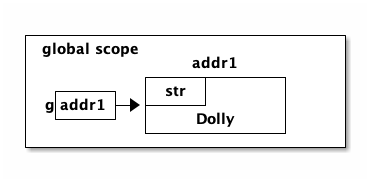
\includegraphics[width=1.75in]{diagrams/dolly.png}
\end{center}

\begin{itemize}
\item Is \texttt{g} a good variable name here?
\end{itemize}
\end{block}
\end{column}

\begin{column}{0.3\columnwidth}
\begin{block}{}
\lstset{language=Python,label= ,caption= ,captionpos=b,numbers=none}
\begin{lstlisting}
>>> greet(g)
\end{lstlisting}

Passes argument \texttt{g} \emph{by value}, that is, the object pointer in \texttt{g} is copied to \texttt{greet}'s \texttt{name} parameter.

\begin{center}
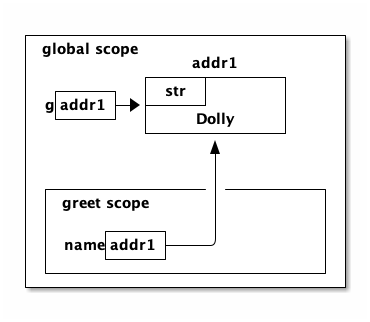
\includegraphics[width=1.75in]{diagrams/greet-dolly.png}
\end{center}
\end{block}
\end{column}


\begin{column}{0.3\columnwidth}
\begin{block}{}
\lstset{language=Python,label= ,caption= ,captionpos=b,numbers=none,basicstyle=\ttfamily\scriptsize, numbers=left}
\begin{lstlisting}
def greet(name):
    g = "Hello, "+name+"!"
    print(g)
\end{lstlisting}

Notice that \texttt{greet}'s \texttt{g} shadows the global \texttt{g}.
\begin{center}
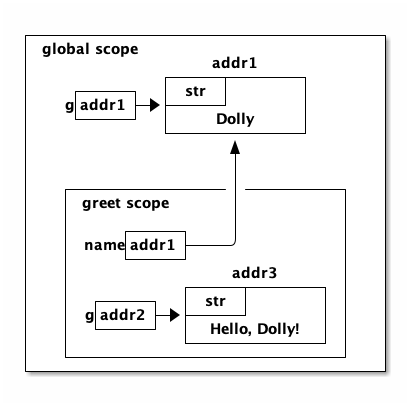
\includegraphics[width=1.75in]{diagrams/greet-scope.png}
\end{center}
\end{block}
\end{column}
\end{columns}
\end{frame}


\begin{frame}[label={sec:org9f752d9},fragile]{Strict Argument Evaluation}
 Arguments to functions are evaluated strictly, meaning that they are evaluated before control is transferred to the function body.

\begin{columns}
\begin{column}{0.3\columnwidth}
\begin{block}{}
\lstset{language=Python,label= ,caption= ,captionpos=b,numbers=none}
\begin{lstlisting}
>>> greet('again')
Guten Tag!
\end{lstlisting}

This creates a temporary \texttt{str} object pointing to the \texttt{Sequence} value \texttt{'again'}

\begin{center}
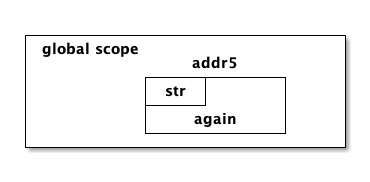
\includegraphics[width=1.75in]{diagrams/again.png}
\end{center}
\end{block}
\end{column}

\begin{column}{0.3\columnwidth}
\begin{block}{}
and passes a reference to that object to the function.

\begin{center}
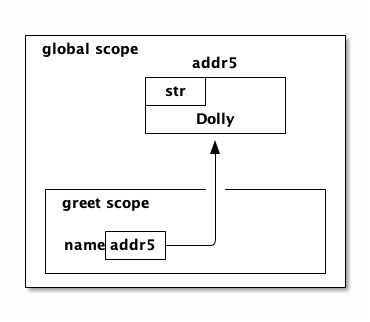
\includegraphics[width=1.75in]{diagrams/greet-again.png}
\end{center}
\end{block}
\end{column}


\begin{column}{0.3\columnwidth}
\begin{block}{}
\lstset{language=Python,label= ,caption= ,captionpos=b,numbers=none,basicstyle=\ttfamily\scriptsize, numbers=left}
\begin{lstlisting}
def greet(name):
    g = "Hello, "+name+"!"
    print(g)
\end{lstlisting}

Then, as before, the local \texttt{g} object is created.

\begin{center}
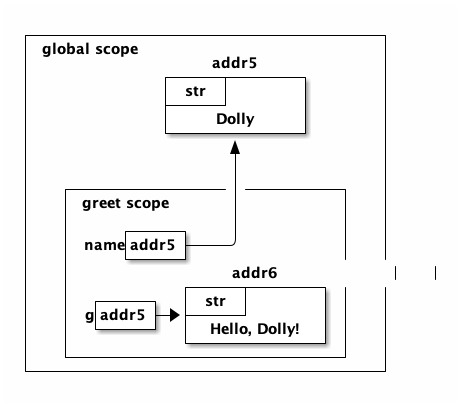
\includegraphics[width=1.75in]{diagrams/greet-again-scope.png}
\end{center}
\end{block}
\end{column}
\end{columns}
\end{frame}



\begin{frame}[label={sec:org85a4f36},fragile]{Variable Scope}
 Parameters are local variables. They are not visible outside the function:

\lstset{language=Python,label= ,caption= ,captionpos=b,numbers=none}
\begin{lstlisting}
>>> name
Traceback (most recent call last):
  File "<stdin>", line 1, in <module>
NameError: name 'name' is not defined
\end{lstlisting}

Global variables are visible outside the function and inside the function.

\lstset{language=Python,label= ,caption= ,captionpos=b,numbers=none}
\begin{lstlisting}
>>> global_hello = 'Bonjour'
>>> global_hello
'Bonjour'
>>> def say_global_hello():
...     print(global_hello)
...
>>> say_global_hello()
Bonjour
\end{lstlisting}
\end{frame}

\begin{frame}[label={sec:org5237da5},fragile]{Shadowing Global Variables}
 Local variables shadow global variables.

\lstset{language=Python,label= ,caption= ,captionpos=b,numbers=none}
\begin{lstlisting}
>>> x = 1
>>> def f():
...     x = 2
...     print("local x:", x)
...     print("global x:", globals()["x"])
...
>>> f()
local x: 2
global x: 1
\end{lstlisting}

\begin{itemize}
\item Tip: evaluate \texttt{globals()["\_\_name\_\_"]} in the Python REPL.
\end{itemize}

A function parameter is a local variable.

\lstset{language=Python,label= ,caption= ,captionpos=b,numbers=none}
\begin{lstlisting}
>>> name = 'Hi ya!'
>>> def greet(name):
...     print(name)
...
>>> name
'Hi ya!'
>>> greet('Hello')
Hello
\end{lstlisting}
\end{frame}

\begin{frame}[label={sec:orgc97c6b5},fragile]{Namespaces}
 Every place where a variable can be defined is called a \alert{namespace} or a \alert{frame} (sometimes also called a \alert{symbol table}, which is how namespaces are implemented by compilers and interpreters).

\begin{itemize}
\item Top level, or \alert{global} names (either the Python REPL or a script) are in a namespace called \texttt{\_\_main\_\_}.
\item Each function \alert{call} also gets a namespace for the local variables in the function.
\item These namespaces are hierarchical -- name resolution starts with the innermost namespace, which is why local variables "hide" or "shadow" global variables.
\end{itemize}
\end{frame}

\begin{frame}[label={sec:org6959aeb},fragile]{Redefining Names}
 A function a kind of variable. If you define a function with the same name as a variable, it re-binds the name, and vice-versa.

\lstset{language=Python,label= ,caption= ,captionpos=b,numbers=none}
\begin{lstlisting}
>>> global_hello = 'Bonjour'
>>> def global_hello():
...     print('This is the global_hello() function.')
...
>>> global_hello
<function global_hello at 0x10063b620>
\end{lstlisting}
\end{frame}

\begin{frame}[label={sec:org9e3176c}]{Python Scope Gotchas}
Python has notoriously weird scoping rules.
\end{frame}

\begin{frame}[label={sec:org197a35e},fragile]{Muliple Parameters}
 A function can take any number of parameters.

\lstset{language=Python,label= ,caption= ,captionpos=b,numbers=none}
\begin{lstlisting}
>>> def greet(greeting, name):
...     print(greeting + ', ' + name)
...
>>> greet('Greetings', 'Professor Falken')
Greetings, Professor Falken
\end{lstlisting}

Parameters can be of multiple types.

\lstset{language=Python,label= ,caption= ,captionpos=b,numbers=none}
\begin{lstlisting}
>>> def greet(name, name, number):
...     print(name * number + ', ' + name)
...
>>> greet('Professor Falken', 'Greetings', 2)
GreetingsGreetings, Professor Falken
\end{lstlisting}
\end{frame}

\begin{frame}[label={sec:org7ee81fe},fragile]{Positional and Keyword Arguments}
 Thus far we've called functions using positional arguments, meaning that argument values are bound to parameters in the order in which they appear in the call.

\lstset{language=Python,label= ,caption= ,captionpos=b,numbers=none}
\begin{lstlisting}
>>> def greet(greeting, name, number):
...     print((greeting + ', ' + name) * 2)
...
>>> greet('Professor Falken', 'Greetings', 2)
\end{lstlisting}

We can also call functions with keyword arguments in any order.

\lstset{language=Python,label= ,caption= ,captionpos=b,numbers=none}
\begin{lstlisting}
>>> greet(greeting='Hello', number=2, name='Dolly')
Hello, DollyHello, Dolly
\end{lstlisting}

If you call a function with both positional and keyword arguments, the positional ones must come first.
\end{frame}

\begin{frame}[label={sec:orge6bf364},fragile]{Default Parameter Values}
 You can specify default parameter values so that you don't have to provide an argument.

\lstset{language=Python,label= ,caption= ,captionpos=b,numbers=none}
\begin{lstlisting}
>>> def greet(greeting, name='Elmo'):
...     print(greeting + ', ' + name)
...
>>> greet('Hello')
Hello, Elmo
\end{lstlisting}

If you provide an argument for a parameter with a default value, the parameter takes the argument value passed in the call instead of the default value.

\lstset{language=Python,label= ,caption= ,captionpos=b,numbers=none}
\begin{lstlisting}
>>> greet('Hi', 'Guy')
Hi, Guy
\end{lstlisting}
\end{frame}

\begin{frame}[label={sec:orgafee6e7},fragile]{Return Values}
 Functions return values.

\lstset{language=Python,label= ,caption= ,captionpos=b,numbers=none}
\begin{lstlisting}
>>> def double(num):
...     return num * 2
...
>>> double(2)
4
\end{lstlisting}

If you don't explicitly return a value, \texttt{None} is returned implicitly.

\lstset{language=Python,label= ,caption= ,captionpos=b,numbers=none}
\begin{lstlisting}
>>> def g():
...     print("man") # This is not a return!
...
>>> fbi = g()
man # This is a side-effect of calling g(), not a return value
>>> type(fbi)
<class 'NoneType'>
\end{lstlisting}

Function calls are expressions like any other, that is, a function call has a value, so a function call can appear anywhere a value can appear.

\lstset{language=Python,label= ,caption= ,captionpos=b,numbers=none}
\begin{lstlisting}
>>> double(2) + double(3)
10
\end{lstlisting}
\end{frame}


\begin{frame}[label={sec:org9648bbb},fragile]{Variable Argument Lists}
 You can collect a variable number of positional arguments as a tuple by preprending a parameter name with \texttt{*}

\lstset{language=Python,label= ,caption= ,captionpos=b,numbers=none}
\begin{lstlisting}
>>> def echo(*args):
...     print(args)
...
>>> echo(1, 'fish', 2, 'fish')
(1, 'fish', 2, 'fish')
\end{lstlisting}

You can collect variable keyword arguments as a dictionary with \texttt{**}

\lstset{language=Python,label= ,caption= ,captionpos=b,numbers=none}
\begin{lstlisting}
>>> def print_dict(**kwargs):
...     print(kwargs)
...
>>> print_dict(a=1, steak='sauce')
{'a': 1, 'steak': 'sauce'}
\end{lstlisting}

And you can do both, but the keword arguments come second.

\lstset{language=Python,label= ,caption= ,captionpos=b,numbers=none}
\begin{lstlisting}
>>> def print_stuff(*args, **kwargs):
...     print(args, kwargs)
...
>>> print_stuff("Pass", "the", a=1, steak='sauce')
{'a': 1, 'steak': 'sauce'}
\end{lstlisting}

\begin{block}{Active Review}
\begin{itemize}
\item What happens when you evaluate

\lstset{language=Python,label= ,caption= ,captionpos=b,numbers=none}
\begin{lstlisting}
  print_stuff("Pass", a=1, steak='sauce', 'the')
\end{lstlisting}
\end{itemize}
\end{block}
\end{frame}

\begin{frame}[label={sec:org55150e0},fragile]{Inner Functions}
 Information hiding is a general principle of software engineering. If you only need a function in one place, inside another function, you can declare it inside that function so that it is visible only in that function.

\lstset{language=Python,label= ,caption= ,captionpos=b,numbers=none}
\begin{lstlisting}
def factorial(n):
   def fac_iter(n, accum):
       if n <= 1:
           return accum
       return fac_iter(n - 1, n * accum)
   return fac_iter(n, 1)

>>> factorial(5)
120
\end{lstlisting}

\texttt{fac\_iter()} is a (tail) recursive function. Recursion is important for computer scientists, but a practically-oriented Python-programming engineer will mostly use iteration, higher-order functions and loops, which are more \href{http://neopythonic.blogspot.com/2009/04/tail-recursion-elimination.html}{Pythonic}. Any recursive computation can be formulated as an imperative computation.

\begin{block}{Active Review}
\begin{itemize}
\item Define the \texttt{factorial} function above in your REPL and evaluate the following calls:

\lstset{language=Python,label= ,caption= ,captionpos=b,numbers=none}
\begin{lstlisting}
  factorial(10)
  factorial(100)
  factorial(1000)
  factorial(10000)
\end{lstlisting}
\end{itemize}
\end{block}
\end{frame}

\begin{frame}[label={sec:orgdb0ca43}]{Conclusion}
\begin{itemize}
\item Functions are the primary way we break a program into reusable pieces.
\item Use functions liberally.
\end{itemize}
\end{frame}
\end{document}